\begin{figure}[H]	
  \centering
    \resizebox{\linewidth}{!}{\tikzset{font=\Huge}\documentclass{standalone}
\usepackage{tikz}
\usepackage{aeguill}
\begin{document}
% generated by Plantuml 1.2018.12      
\definecolor{plantucolor0000}{RGB}{254,254,206}
\definecolor{plantucolor0001}{RGB}{168,0,54}
\definecolor{plantucolor0002}{RGB}{173,209,178}
\definecolor{plantucolor0003}{RGB}{0,0,0}
\definecolor{plantucolor0004}{RGB}{180,167,229}
\begin{tikzpicture}[yscale=-1
,pstyle0/.style={color=plantucolor0001,fill=plantucolor0000,line width=1.5pt}
,pstyle1/.style={color=plantucolor0001,fill=plantucolor0002,line width=1.0pt}
,pstyle2/.style={color=plantucolor0001,line width=1.5pt}
,pstyle4/.style={color=plantucolor0001,line width=1.0pt}
,pstyle5/.style={color=plantucolor0001,fill=plantucolor0001,line width=1.0pt}
]
\draw[pstyle0] (6pt,8pt) rectangle (130.9098pt,81.6094pt);
\draw[pstyle1] (37.7894pt,24pt) ellipse (11pt and 11pt);
\node at (37.7894pt,24pt)[]{\textbf{\Large C}};
\node at (55.5204pt,17.0156pt)[below right,color=black]{Context};
\draw[pstyle2] (7pt,40pt) -- (129.9098pt,40pt);
\node at (12pt,44pt)[below right,color=black]{strategy};
\draw[pstyle2] (7pt,60.8047pt) -- (129.9098pt,60.8047pt);
\node at (12pt,64.8047pt)[below right,color=black]{+contextMethod()};
\draw[pstyle0] (166pt,14.5pt) rectangle (286.9773pt,75.3047pt);
\draw[color=plantucolor0001,fill=plantucolor0004,line width=1.0pt] (193.7783pt,30.5pt) ellipse (11pt and 11pt);
\node at (193.7783pt,30.5pt)[]{\textbf{\Large I}};
\node at (210.6179pt,23.5156pt)[below right,color=black]{\textit{Strategy}};
\draw[pstyle2] (167pt,46.5pt) -- (285.9773pt,46.5pt);
\draw[pstyle2] (167pt,54.5pt) -- (285.9773pt,54.5pt);
\node at (172pt,58.5pt)[below right,color=black]{\textit{strategyMethod()}};
\draw[pstyle0] (42pt,142pt) rectangle (208.8552pt,202.8047pt);
\draw[pstyle1] (57pt,158pt) ellipse (11pt and 11pt);
\node at (57pt,158pt)[]{\textbf{\Large C}};
\node at (71pt,151.0156pt)[below right,color=black]{ConcreteStrategy1};
\draw[pstyle2] (43pt,174pt) -- (207.8552pt,174pt);
\draw[pstyle2] (43pt,182pt) -- (207.8552pt,182pt);
\node at (48pt,186pt)[below right,color=black]{-strategyMethod()};
\draw[pstyle0] (244pt,142pt) rectangle (410.8552pt,202.8047pt);
\draw[pstyle1] (259pt,158pt) ellipse (11pt and 11pt);
\node at (259pt,158pt)[]{\textbf{\Large C}};
\node at (273pt,151.0156pt)[below right,color=black]{ConcreteStrategy2};
\draw[pstyle2] (245pt,174pt) -- (409.8552pt,174pt);
\draw[pstyle2] (245pt,182pt) -- (409.8552pt,182pt);
\node at (250pt,186pt)[below right,color=black]{-strategyMethod()};
\draw[pstyle4] (144.4055pt,45pt) ..controls (147.1893pt,45pt) and (149.9732pt,45pt) .. (152.757pt,45pt);
\draw[pstyle5] (165.7854pt,45pt) -- (156.7854pt,41pt) -- (160.7854pt,45pt) -- (156.7854pt,49pt) -- (165.7854pt,45pt) -- cycle;
\draw[pstyle4] (160.7854pt,45pt) -- (152.7854pt,44.9999pt);
\draw[pstyle5] (131.1445pt,45pt) -- (137.1445pt,49pt) -- (143.1445pt,45pt) -- (137.1445pt,41pt) -- (131.1445pt,45pt) -- cycle;
\draw[pstyle4] (189.8575pt,91.2566pt) ..controls (176.5428pt,108.0648pt) and (161.8351pt,126.6314pt) .. (149.8447pt,141.7679pt);
\draw[pstyle4] (184.4021pt,86.87pt) -- (202.308pt,75.5394pt) -- (195.3762pt,95.5632pt) -- (184.4021pt,86.87pt) -- cycle;
\draw[pstyle4] (263.1425pt,91.2566pt) ..controls (276.4572pt,108.0648pt) and (291.1649pt,126.6314pt) .. (303.1553pt,141.7679pt);
\draw[pstyle4] (257.6238pt,95.5632pt) -- (250.692pt,75.5394pt) -- (268.5979pt,86.87pt) -- (257.6238pt,95.5632pt) -- cycle;
\end{tikzpicture}
\end{document}
}
\end{figure}
\begin{intentbox}[Intent]\nospacing
  \begin{itemizenosep}
      \item Allow to change algorithms independently of the clients
      \item Support extensibility with new algorithms
      \item Make algorithms interchangeable
  \end{itemizenosep}
\end{intentbox}
\begin{sectionbox}[Which problem does it solve]\nospacing
  \begin{minipage}[t]{0.45\textwidth}
  Strategy pattern is an alternative to specialization of context
  class which:
  \begin{itemizenosep}
      \item violates the \rd{Single Responsibility Principle}
      \item prevents interchanging the strategy of a context dynamically, as
    subclassing statically defines the binding between context and strategy
  \end{itemizenosep}
  \end{minipage}
  \begin{minipage}[t]{0.5\textwidth}
  \begin{figure}[H]
    \centering
    \vspace{-1em}
      \resizebox{\linewidth}{!}{\documentclass{standalone}
\usepackage{tikz}
\usepackage{aeguill}
\begin{document}
% generated by Plantuml 1.2018.12      
\definecolor{plantucolor0000}{RGB}{254,254,206}
\definecolor{plantucolor0001}{RGB}{168,0,54}
\definecolor{plantucolor0002}{RGB}{173,209,178}
\definecolor{plantucolor0003}{RGB}{0,0,0}
\begin{tikzpicture}[yscale=-1
,pstyle0/.style={color=plantucolor0001,fill=plantucolor0000,line width=1.5pt}
,pstyle1/.style={color=plantucolor0001,fill=plantucolor0002,line width=1.0pt}
,pstyle2/.style={color=plantucolor0001,line width=1.5pt}
,pstyle3/.style={color=plantucolor0001,line width=1.0pt}
]
\draw[pstyle0] (77pt,8pt) rectangle (164.6pt,68.8047pt);
\draw[pstyle1] (92pt,24pt) ellipse (11pt and 11pt);
\node at (92pt,24pt)[]{\textbf{\Large C}};
\node at (106pt,17.0156pt)[below right,color=black]{Context};
\draw[pstyle2] (78pt,40pt) -- (163.6pt,40pt);
\node at (83pt,44pt)[below right,color=black]{\textit{strategy}};
\draw[pstyle2] (78pt,60.8047pt) -- (163.6pt,60.8047pt);
\draw[pstyle0] (6pt,129pt) rectangle (103.9439pt,189.8047pt);
\draw[pstyle1] (21pt,145pt) ellipse (11pt and 11pt);
\node at (21pt,145pt)[]{\textbf{\Large C}};
\node at (35pt,138.0156pt)[below right,color=black]{ContextA};
\draw[pstyle2] (7pt,161pt) -- (102.9439pt,161pt);
\node at (12pt,165pt)[below right,color=black]{strategy};
\draw[pstyle2] (7pt,181.8047pt) -- (102.9439pt,181.8047pt);
\draw[pstyle0] (139pt,129pt) rectangle (236.593pt,189.8047pt);
\draw[pstyle1] (154pt,145pt) ellipse (11pt and 11pt);
\node at (154pt,145pt)[]{\textbf{\Large C}};
\node at (168pt,138.0156pt)[below right,color=black]{ContextB};
\draw[pstyle2] (140pt,161pt) -- (235.593pt,161pt);
\node at (145pt,165pt)[below right,color=black]{strategy};
\draw[pstyle2] (140pt,181.8047pt) -- (235.593pt,181.8047pt);
\draw[pstyle3] (94.605pt,86.8909pt) ..controls (86.8583pt,101.0932pt) and (78.6053pt,116.2237pt) .. (71.6493pt,128.9764pt);
\draw[pstyle3] (88.623pt,83.2393pt) -- (104.3454pt,69.0334pt) -- (100.9136pt,89.9433pt) -- (88.623pt,83.2393pt) -- cycle;
\draw[pstyle3] (147.795pt,86.8909pt) ..controls (155.659pt,101.0932pt) and (164.0371pt,116.2237pt) .. (171.0985pt,128.9764pt);
\draw[pstyle3] (141.4714pt,89.9211pt) -- (137.9069pt,69.0334pt) -- (153.7191pt,83.1393pt) -- (141.4714pt,89.9211pt) -- cycle;
\end{tikzpicture}
\end{document}
}
  \end{figure}
  \end{minipage}
\end{sectionbox}
\begin{partbox}[Participants]\nospacing
  \begin{itemizenosep}
      \item \imp{Context}: 
      is the real thing e.g.\
      \begin{itemize}
          \item A secure channel
          \item Container
          \item TransportationToAirport
      \end{itemize}
      that uses a concrete strategy.\\
      Thus it must have a reference/stores an instance of the concrete strategy.\\
      The name of the context method(s) depends on the context e.g.\
      \begin{itemize}
          \item encrypt, decrypt
          \item addLayoutComponent, minimumLayoutSize
          \item transport
      \end{itemize}
      and acts depending on it by calling the \javainline{request} or \javainline{doAction} method of its current state reference.
      \item \imp{Strategy/Algorithm Interface}: is
        usually an interface as we implement some functionality and do not have an
        ``is-a'' relationship.\\
        The strategy interface specifies which methods the algorithms may be
        able to perform.
    \item \imp{Concrete Algorithm}: Implements the methods of the \textit{Strategy interface}
  \end{itemizenosep}
\end{partbox}
\begin{notebox}[Note]\nospacing
  \begin{itemizenosep}
    \item Strategy methods may contain a \ul{reference} to the context as a parameter,
  in order to use a state full algorithm see
  \cref{subsubsec:statefullVsStateless}.
    \item Strategy Interface may be defined inside the context class.
  \end{itemizenosep}
\end{notebox}
\begin{codeboxNl}[Context]{java}
  class Context{
    private Strategy algorithm;
    
    public void setAlgorithm(Strategy a){
      if(a == 0){ // See also Null Object Pattern |\cref{subsubsec:NullObjectPattern}|
        throw new IllegalArgumentException();
      } 
      this.algorithm = a;
    }

    public State contextMethod1(){
      algorithm.doAction1()
    }

    public State contextMethod1(){
      algorithm.doAction1()
      algorithm.doAction2(|\ul{\opta{this}}|,|\optc{args}|)
      algorithm.doAction1()
    }

  }
\end{codeboxNl}
\begin{codeboxNl}[Strategy Interface]{java}
  interface class Strategy {
    privat void doAction1();
    privat void doAction2(|\ul{\opta{Context cur}}|,|\optc{args}|);
}
\end{codeboxNl}
\begin{codeboxNl}[Concrete Strategy]{java}
  class Algorithm1 implements Strategy {
    privat void doAction1(){|\ldots|};
    privat void doAction2(|\ul{\opta{Context cur}}|,|\optc{args}|){|\ldots|};
}
\end{codeboxNl}
\subsubsection{Statefull vs Stateless Strategys}
\label{subsubsec:statefullVsStateless}
\begin{sectionbox}\nospacing
\begin{figure}[H]
  \centering
  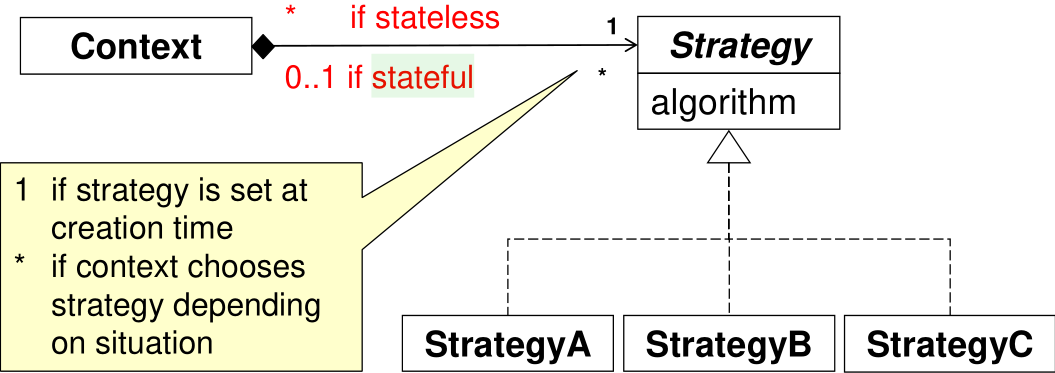
\includegraphics[width=1.0\columnwidth]{figures/strategyStatefulVsStateless.png}
  \label{fig:StatefullVsStateless}
\end{figure}
 \begin{itemizenosep}
     \item \rdb{Stateless} Strategy: does not store/have any state/context
   specific parameters $\Rightarrow$ strategy can be used from different
   contexts.\\
   \imp{Note}: in order to use parameters, strategy may \ul{access} state
   specific parameters of \textit{context} (but not itself!).
     \item \rdb{Statefull} Strategy: may store/have any state/context specific
   parameters $\Rightarrow$ cannot be exchanged between different contexts.
 \end{itemizenosep} 
\end{sectionbox}
\begin{sectionbox}[Strategy vs. State]\nospacing
\begin{minipage}[t]{0.45\textwidth}
  \imp{\tc{section}{Strategy}}
  \begin{itemize}
    \item Strategy is typically not aware of other concrete strategies
    \item Typically set only once
    \item Usually only one \textit{public} method
    \item Strategy may contain algorithm specific state
  \end{itemize}
\end{minipage}
\begin{minipage}[t]{0.45\textwidth}
  \imp{\tc{section}{State}}
  \begin{itemize}
      \item A concrete state may be aware of others $\Rightarrow$ transitions.
      \item Defines state-specific behavior
      \item Typically state changes at runtime
      \item State usually contains no state but accesses state in context
  \end{itemize}
\end{minipage}
\end{sectionbox}
%%% Local Variables:
%%% mode: latex
%%% TeX-master: "../formulary"
%%% End:
